\documentclass[12pt,a4paper]{book}
\usepackage[utf8]{inputenc}
\usepackage{amsmath}
\usepackage{amsfonts}
\usepackage{amssymb}
\usepackage{graphicx}
\usepackage{draftwatermark}
\usepackage{textcomp}
\date{07-09-2018}
\author{Philip Martin Taylor}
\title{TaylorWorld Leaflet}
\begin{document}
\begin{center}
\textbf{Welcome to TaylorWorld \texttrademark.}
\end{center}
\begin{figure}[h]
  \centering
  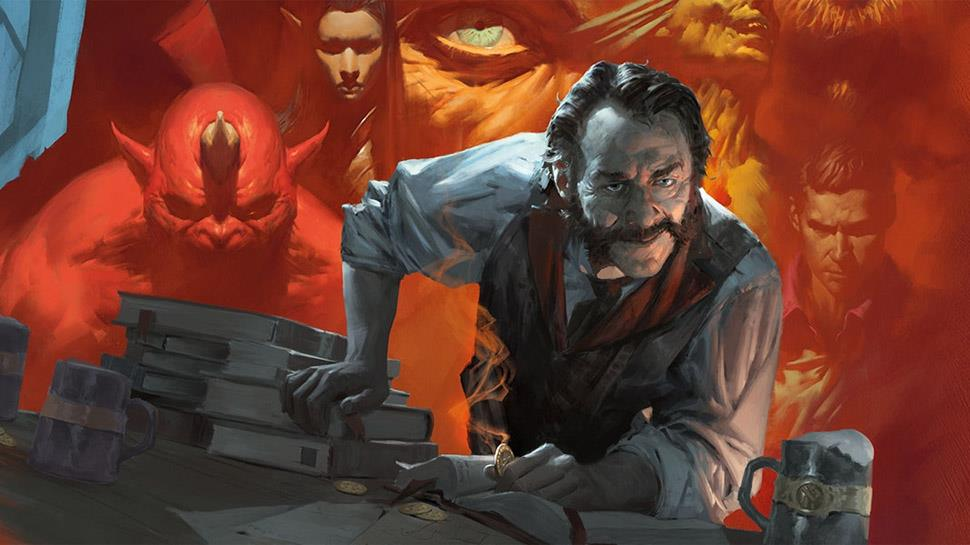
\includegraphics[scale=0.15]{alchemist.jpg}
  %\caption{Lego Wizard}
\end{figure}
\begin{flushleft}
We are experts in the RPG's, Dungeons and Dragons, Pathfinder and Starfinder. Our website is https://taylorworld.one and our contact email is ptaylor@taylorworld.one.
\end{flushleft}
\begin{flushleft}
  If you see this leaftlet and your interested in exploring these games, either email us, show your interest in the Bailiff's Tap or leave a message on our Facebook page https://www.facebook.com/brobostigon/ .
\end{flushleft}
\begin{flushleft}
  We do taster sessions and other kinds of gaming events at the Bailiffs Tap in Banbury, Oxfordshire, where you can come and get reacquainted with the RPG's you love and remember.
\end{flushleft}
\begin{flushleft}
  Pathfinder and 'Dungeons and Dragons' are traditional D20 based, medieval setting RPG's. Starfinder is equally a D20 based RPG, however as its based in the future it has significant differences, including a variety of different charecter races, which include the Android, and a veriety of different charecter classes, which include the Technomancer. Starfinder also includes things like Laser Pistols, StarShips, cybernetic enhancements and different ways of casting magic.
\end{flushleft}
\begin{center}
  \textcopyright{} 2018 Philip Martin Taylor.
\end{center}
\begin{center}
  Pathfinder and Starfinder are Registered Trademarks of Paizo Publishing LLC. Dungeons and Dragons is a Registered Trademark of Wizards of the Coast LLC.
\end{center}
\end{document}
